\chapter{Introduction}
\label{chap:ch1}

\section{About}
\label{chap:ch1sec1}

\par Emulators play a vital role in computing by enabling software to run on hardware or virtual platforms distinct from their original execution environments.

\par Their applications span a wide range of domains, including legacy video game preservation, processor simulation, and the development of sandboxed runtime systems.

\par Two fundamental techniques underpin most emulator implementations: interpretation and just-in-time (JIT) compilation.

\par A clear understanding of the strengths and limitations of these approaches is crucial for those engaging in low-level systems development or virtual machine construction.

\par This thesis offers an introductory exploration of interpretation and JIT compilation, supported by practical implementation and performance analysis.

\par To illustrate these techniques in a manageable and pedagogically valuable context, the study focuses on two minimal programming languages: Brainfuck and CHIP-8.

\par Brainfuck, a minimalist yet Turing-complete esoteric language, and CHIP-8, a simple virtual machine historically used for teaching early computing and game development concepts, serve as effective case studies due to their simplicity and well-defined behavior.

\par The primary objectives of this thesis are as follows:

\begin{itemize}
	\item To implement both interpreters and JIT compilers for Brainfuck and CHIP-8.
	\item To explore and apply basic runtime optimizations.
	\item To compare the performance and complexity of each technique using a set of representative benchmark programs.
	\item To explore application design by creating a proper modularised architecture which is unit and integration tested.
\end{itemize}

\par This thesis aims to provide readers with both a conceptual and practical understanding of how various emulation techniques perform and operate under comparable conditions.

\par The organization of the thesis is outlined as follows:

\begin{itemize}
    \item \textbf{Chapter 2} examines the Brainfuck programming language, focusing on its implementation through both interpretation and just-in-time (JIT) compilation, along with a comparative analysis of their respective performance characteristics.
    \item \textbf{Chapter 3} explores the historical evolution and variations of the CHIP-8 virtual machine, detailing the implementation strategies adopted in this thesis and their implications for emulator design.
    \item \textbf{Chapter 4} provides an in-depth analysis of the modular architecture of the main application, describing the integration and interaction of its components and the rationale behind key design decisions.
    \item \textbf{Chapter 5} summarizes the core findings of the study, discusses its limitations, and proposes potential directions for future research and development in the field of software emulation.
\end{itemize}

\section{Related work}
\label{chap:ch1sec2}

\par CHIP-8 Applications in engineering \cite{Chip8Applications2019}.
Brainfuck in reinforcement learning \cite{BFReinforcementLearining2022}.
Esoteric languages list with BF in it \cite{BFEsolang2015}.
Brainfuck conceputal \cite{BFConceptual2017}.
Brainfuck hardware \cite{BFHardware2016}.
Brainfuck self interpreter \cite{BFSelfInterpreter2003}.

\begin{figure}[htbp]
	\centering
		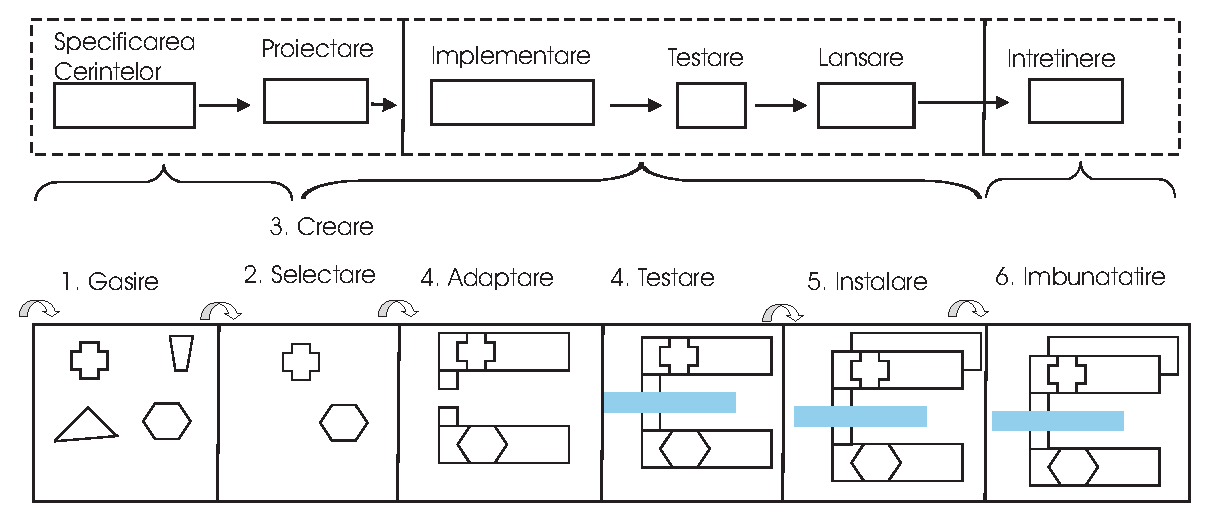
\includegraphics[scale=0.65]{./figures/fig_3_1.eps}
	\caption{Ciclul de dezvoltare al sistemelor bazate pe componente adaptat modelului cascadã}
	\label{FigCBSD}
\end{figure}

Inserarea și Referirea la Tabelul \ref{TabelSolutii}. 

\begin{table}[htbp]
\begin{center}
\begin{tabular}
{|p{120pt}|p{120pt}|p{120pt}|}
\hline
 Nume algoritm  &  Toate soluțiile &  Soluția optimã\\
\hline 
\hline Nume 1 & $20$ & $5$  \\
\hline Nume 2 & $20$ & $2$  \\
\hline
\end{tabular}
\end{center}
\caption{Soluții obținute }
\label{TabelSolutii}
\end{table}


Adaugarea și Referirea la o Ecuație \ref{LabelMyEquation}.


 \begin{equation}
     ws_N4 = w_{14}*N1 + W_{24}+N2 + w_{34}*N3
\label{LabelMyEquation}
 \end{equation}
